% ************************************************
\chapter{Network Model}\label{ch:Network Model} 
% ************************************************

Referring to anisotropic characteristics in local cortical circuits of
the rat's brain, a network model implementing anisotropic tissue
geometry is developed. The introduction of a rewiring algorithm and
qualitative anisotropy measure %quantitative ??
lay the foundation for the analysis of structural aspects of this
model in Chapter~\ref{ch:structural_aspects}.

\parskip = \baselineskip %??
\setlength{\parindent}{0pt}

\section{Introduction}\label{sec:intro_model}

\section{Anisotropy in rat brain}\label{sec:biol_anisotropy}

Braitenberg and Schüz report \parencite{Braitenberg_Cortex}
\begin{quote}
"The main stem of [a pyramidal cell's] axon almost always takes a
vertical downward course, with little deviation from a straight
line. The same tendency can be seen in the primary and secondary
branches of the axon, which may take off at any angle but tend to keep
their straight course from one point of ramification to the next, or
to the point of termination."
\end{quote}

% The open morphology data base supports 

% figure: showing cells so and so, can confirm claim that axons are
% straight.

\vspace{0.5cm}
\begin{figure}[h] 
  \centering 
  \makebox[0.875\textwidth]{%
    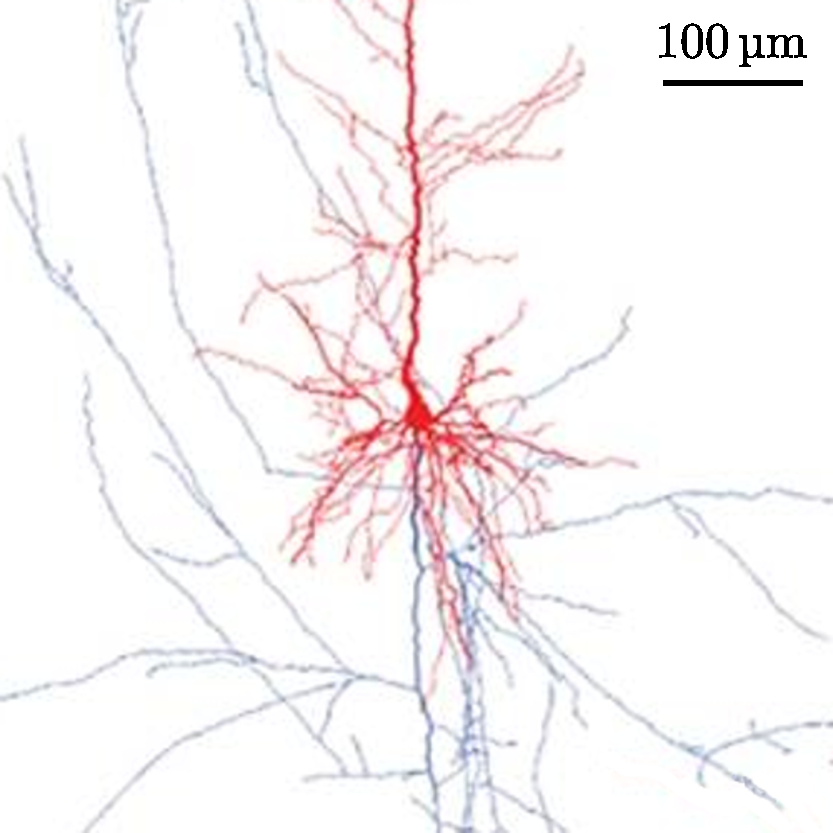
\includegraphics[width=0.4\textwidth]{%
      gfx/img/network_model/p14rr_1_background_unit.pdf}%
    \hfill
    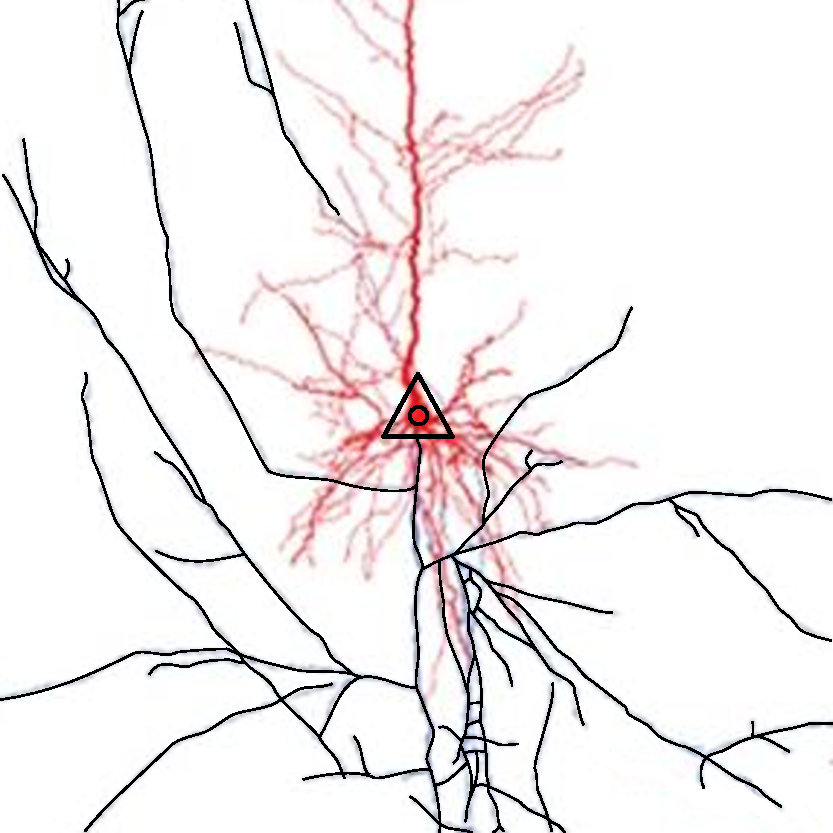
\includegraphics[width=0.4\textwidth]{%
      gfx/img/network_model/p14rr_1_traced_soma_background.pdf}% 
    }%

  \caption{\textbf{Tracing axonal branching of a pyramidal cell} }%??
  \small
  \textbf(A)Using image manipulation software (Inkscape) the The main stem of [a pyramidal cell's] axon almost always takes a
vertical downward course, with little deviation from a straight
line. The same tendency can be seen in the primary and secondary
branches of the axon, which may take off at any angle but tend to keep
their straight course from one point of ramification to the next, or
to the point of termination.
  \textcite{Romand2011}
  \label{fig:romand_traced}
\end{figure}



\vspace{0.5cm}
\begin{figure}[h] 
  \centering 
  \makebox[0.875\textwidth]{%
    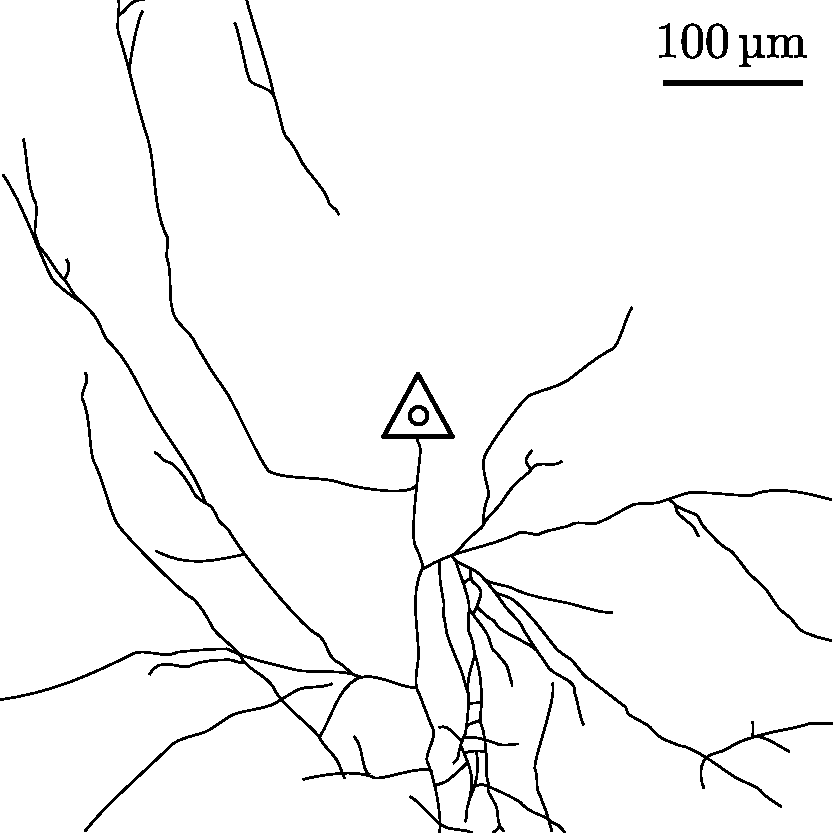
\includegraphics[width=0.4\textwidth]{%
      gfx/img/network_model/p14rr_1_trace_soma.pdf}%
    \hfill
    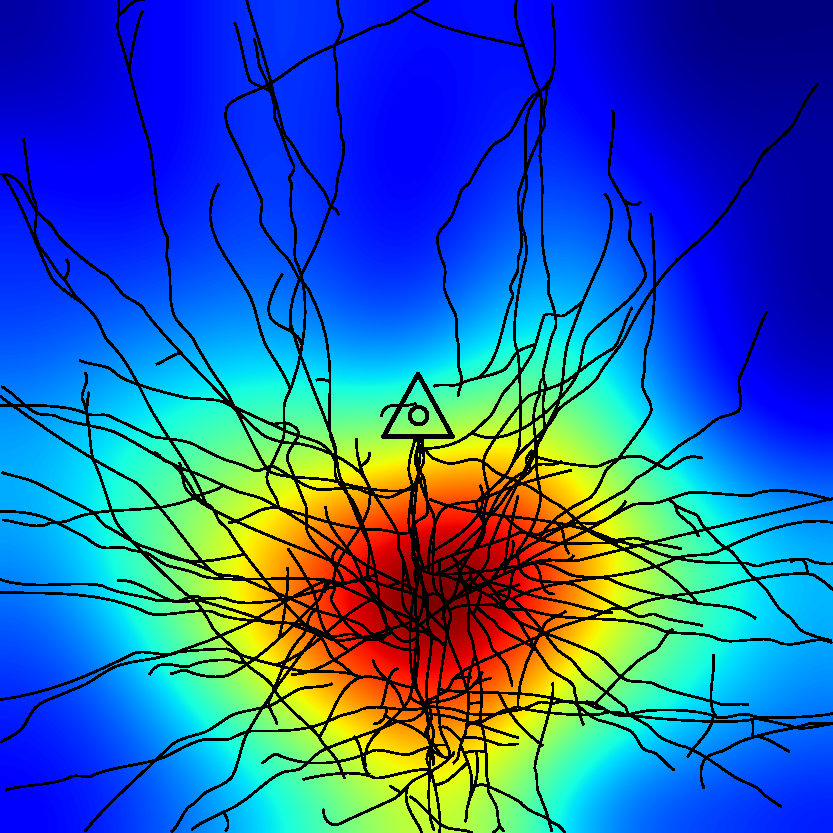
\includegraphics[width=0.4\textwidth]{%
      gfx/img/network_model/heatmap_overlay_png.pdf}% 
    }%
    \caption{\textbf{Overlay of 5 axonal branches}}%??
  \label{fig:axon_heat}
\end{figure}





\newpage
\section{Anisotropic geometric graph model}\label{sec:network_model}

\newpage
\section{Distance dependent connectivity}\label{sec:dist_depend_con}

In Gilbert's random graph model $G(n,p)$, 
\marginpar{Random Graph  Model section~\ref{sec:gilbert_graph}} %?? TITLE
probability of connection $p$ is independently chosen and a fixed
value for all vertex pairs. The anisotropic geometric graph model
introduced in the last %(true??)
section is itself a random graph model - node positions as well as
preferred directions of connection are randomly, uniformly
distributed. In contrast to Gilbert's model however, neither is the
probability of connection between a given vertex pair independent of
the realization of other edges in the graph, nor is it a fixed value -
probabilities strongly depend on internode distance in the
anisotropic geometric graph model introduced.

\vspace{0.5cm}
\begin{figure}[h] 
  \centering 
  \makebox[0.875\textwidth]{%
    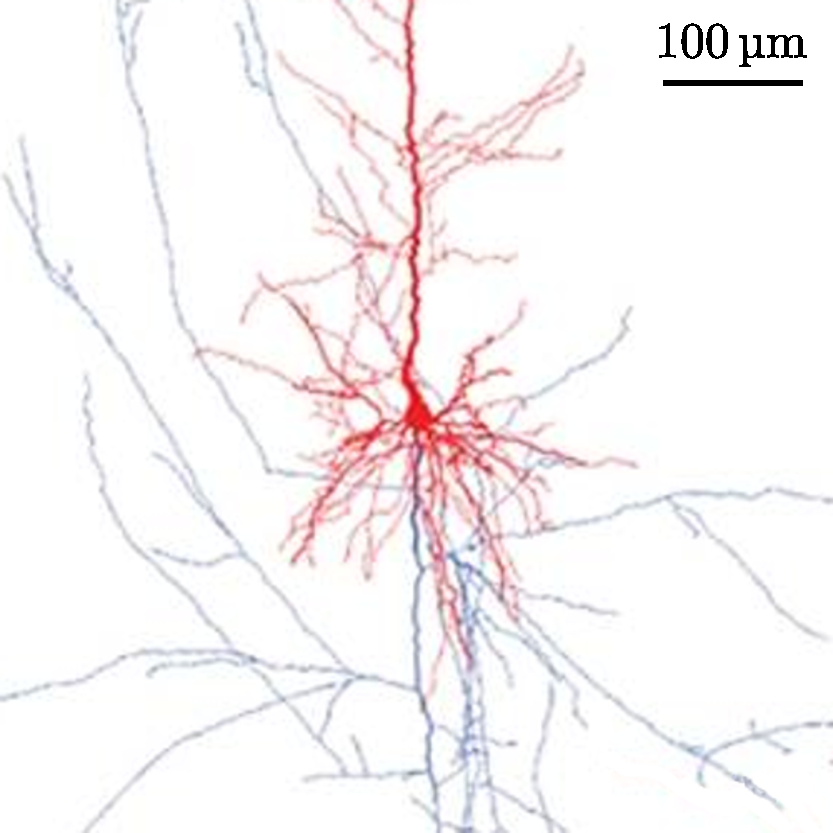
\includegraphics[width=0.4\textwidth]{%
      gfx/img/network_model/p14rr_1_background_unit.pdf}%
    \hfill
    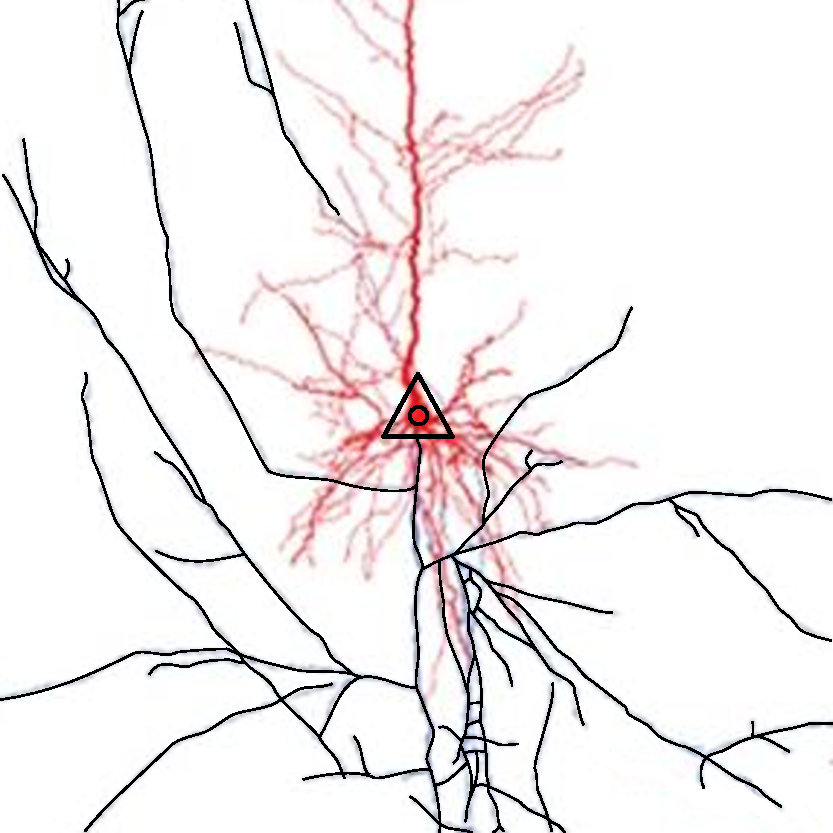
\includegraphics[width=0.4\textwidth]{%
      gfx/img/network_model/p14rr_1_traced_soma_background.pdf}% 
    }%

  \caption{\textbf{Tracing axonal branching of a pyramidal cell}
    \newline 
    thick-tufted layer V pyramidal cell the axon in blue, basal
    dendrites in red.  
    \textbf{(A)} In a \SI{600}{\micro\meter} window around the axon}%
   
  
    % \textb{(B)} 
    % Using image manipulation software (Inkscape)
    
    % \textcite{Romand2011}}%??

 
  \label{fig:romand_traced}
\end{figure}

Analyzing dependencies in the anisotropic model, specifically by
identifying prevalent patterns of connectivity and relating these
modes of non-randomness to biological findings, is the main focus of
Chapter~\ref{ch:structural_aspects}. However, such structural
correlations may not necessarily be an inherent feature of the
network's anisotropy - distance dependent connectivity alone, as
imposed by the model's specific geometry, may be the cause for
emerging dependencies. It is therefore a crucial initial task to map
the anisotropic model's distance dependent connection
probability. Inferring connection probability as a function of
internode distance and comparing it with computational results, in
this section we explore distance connectivity of the anisotropic
network model, securing a vital component in the analysis of
structural features.

Consider a graph $G$. In Gilbert's random graph model the probability
$p$ for a edge between nodes $v,w \in V(G)$ to be realized is a fixed
value; in a geometric graph it is more generally a function of the
distance between the nodes, $d(v,w)$. In short, we write $p(x)$ to
denote the probability that a vertex pair of distance $x$ is
connected,

\[p(x) := P\left[(v,w)|\,d(v,w)=x\right].\]
Owning to the abstract geometric model we defined, this connection
probability is easily computed.

\begin{proposition} %?? make proposition or something
In the anisotropic geometric graph model distance depend connection
probabilities are computed as 
\[
p(x) = \begin{cases} 0.5 & \mathrm{for} \,\, x\le w/2 \\
                       \frac{1}{\pi}
                       \operatorname{arcsin}(\frac{x}{2w}) &
                       \mathrm{for} \,\, x >
                       w/2. \end{cases}
\]
\end{proposition} 

\begin{proof}
  To see this, consider a given source vertex $v$ at $(0,0)$ and a
  possible target $w$, such that $d(v,w) = x$. We may then express the
  target coordinates as $x e^{i\varphi}$, $0 \le \varphi < 2\pi$.

  Figure~\ref{fig:geomtr_prb} illustrates for which angles
  $\varphi$ the node $w$ becomes a valid target for an edge from
  $v$. This intervall

  \begin{figure}[h] 
    \centering 
    \makebox[0.85\textwidth]{%
      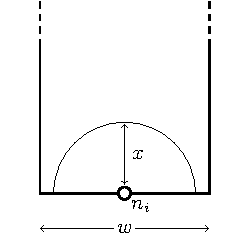
\includegraphics[width=0.4\textwidth]{gfx/tikz/geomtr_prb_05.pdf}%
      \hfill
      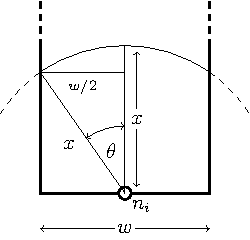
\includegraphics[width=0.4\textwidth]{gfx/tikz/geomtr_prb.pdf}% 
    }%
    %\caption{}%??
    \label{fig:geomtr_prb}
  \end{figure}

  For a general $v$ make coordinate transformation

\end{proof}

We can verify this result by computationally extracting the distance
dependencies in the sample graphs generated. 

\begin{figure}[h]
  \centering
  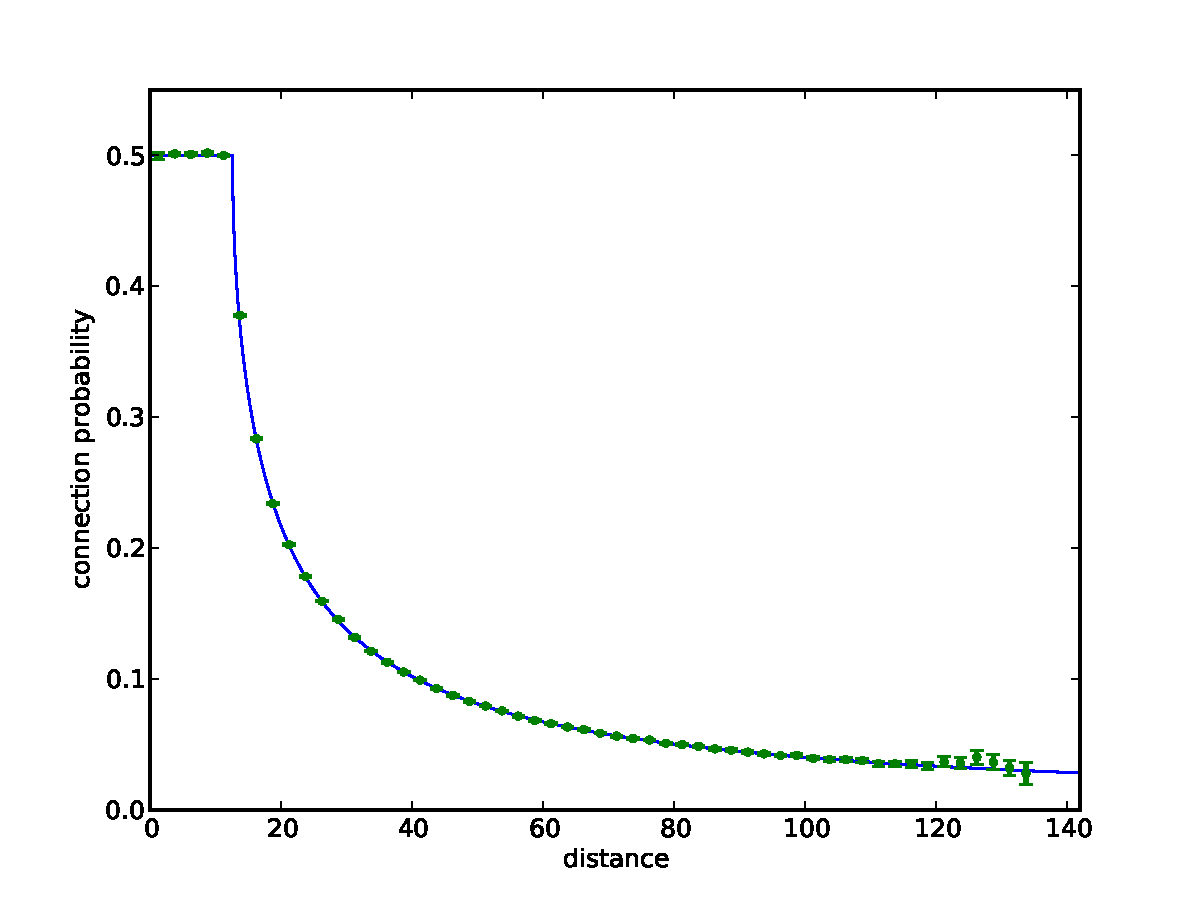
\includegraphics[width=0.7\linewidth]{gfx/plots/test.pdf}
  \caption{\textbf{Distance dependent connection probabilities}}%??
  \label{fig:something_else}%??
\end{figure}





\section{Rewiring Methods}

In the network configuration introduced in
section~\ref{sec:network_model} strong directional anisotropy is
present: Edges originating from one node \enquote{point in the same
  direction}, that is they connect to other nodes which cluster around
a. In this section we introduce an algorithm

\vspace{0.5cm}
\begin{figure}[h] 
  \centering 
  \makebox[0.85\textwidth]{%
    %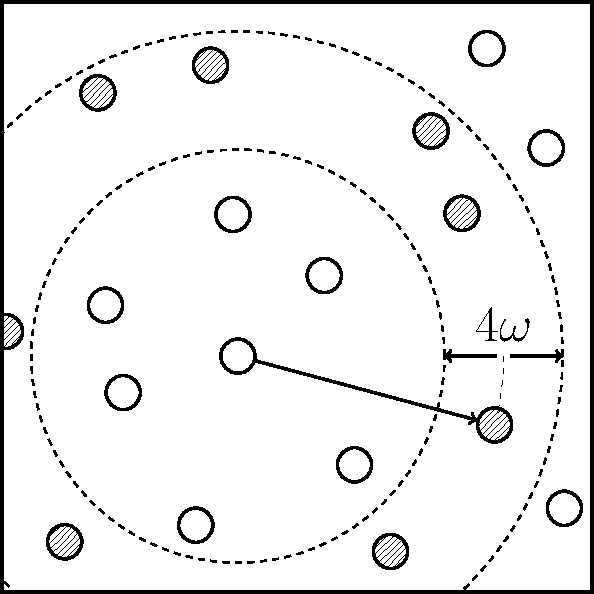
\includegraphics[width=0.4\textwidth]{gfx/dist_rew_org.pdf}%
    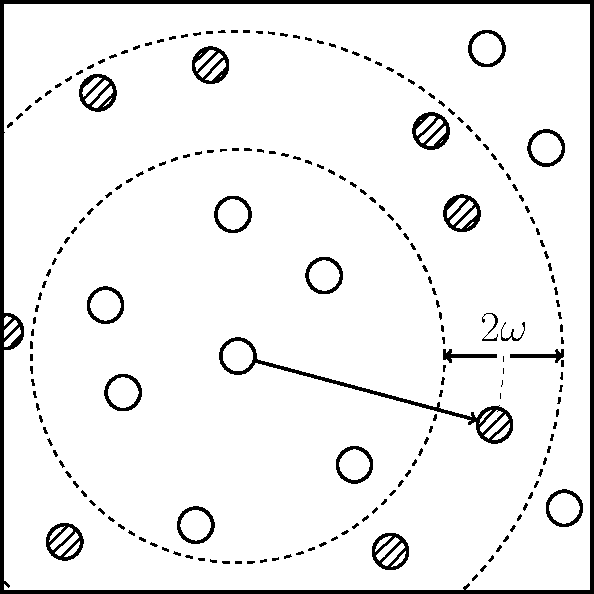
\includegraphics[width=0.4\textwidth]{gfx/tikz/distance_rewiring.pdf}%
    \hfill
    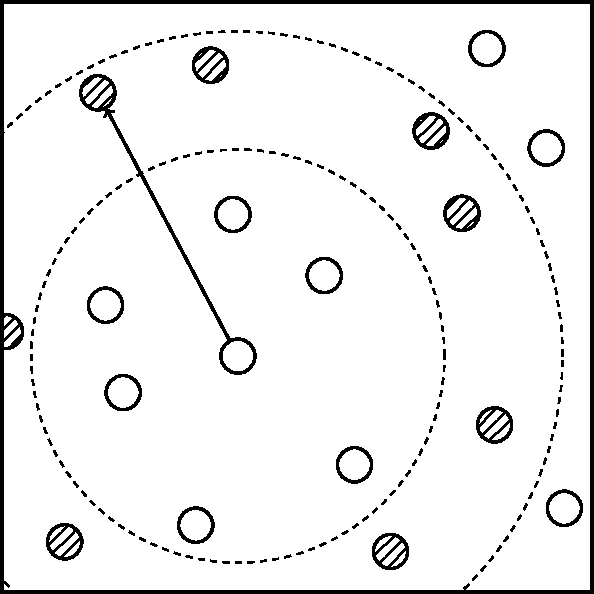
\includegraphics[width=0.4\textwidth]{gfx/dist_rew_rew.pdf}% 
  }%
  \caption{\textbf{Rewiring}}%??
  \label{fig:distance_rewiring}
\end{figure}

 

\section{Anisotropy Measure}


\section{Summary and Discussion}













%%% Local Variables: 
%%% mode: latex
%%% TeX-master: "../ClassicThesis"
%%% End: 
